
% ----------------------------------------------------------------------
%  Set the document class
% ----------------------------------------------------------------------
\documentclass[11pt,a4paper,twoside]{article}

% ----------------------------------------------------------------------
% Define external packages, language, margins, fonts and new commands
% ----------------------------------------------------------------------
%\input{preamble} 
\usepackage[utf8]{inputenc}   % <<<<< Linux
\usepackage[english]{babel} % <<<<< English
\usepackage{notoccite}
\usepackage[skip=0.5\baselineskip]{caption}
\hyphenation{GTKWave}
\usepackage{listings}
\usepackage[all]{nowidow}
\usepackage{float}
\usepackage{tabularx}

%blind text
\usepackage{lipsum}

\usepackage{graphicx}
\graphicspath{ {./} {../../figlib/} }
\def\FontLn{% 16 pt normal
  \usefont{T1}{phv}{m}{n}\fontsize{16pt}{16pt}\selectfont}
\def\FontLb{% 16 pt bold
  \usefont{T1}{phv}{b}{n}\fontsize{16pt}{16pt}\selectfont}
\def\FontMn{% 14 pt normal
  \usefont{T1}{phv}{m}{n}\fontsize{14pt}{14pt}\selectfont}
\def\FontMb{% 14 pt bold
  \usefont{T1}{phv}{b}{n}\fontsize{14pt}{14pt}\selectfont}
\def\FontSn{% 12 pt normal
  \usefont{T1}{phv}{m}{n}\fontsize{12pt}{12pt}\selectfont}

% Use Arial font as default
%
\renewcommand{\rmdefault}{phv}
\renewcommand{\sfdefault}{phv}
\usepackage{geometry}	
\geometry{verbose,tmargin=2.5cm,bmargin=2.5cm,lmargin=2.5cm,rmargin=2.5cm}

%\usepackage{setspace}
%\renewcommand{\baselinestretch}{1.5}

\usepackage[pdftex]{hyperref} % enhance documents that are to be
                              % output as HTML and PDF
\hypersetup{colorlinks,       % color text of links and anchors,
                              % eliminates borders around links
%            linkcolor=red,    % color for normal internal links
            linkcolor=black,  % color for normal internal links
            anchorcolor=black,% color for anchor text
%            citecolor=green,  % color for bibliographical citations
            citecolor=black,  % color for bibliographical citations
%            filecolor=magenta,% color for URLs which open local files
            filecolor=black,  % color for URLs which open local files
%            menucolor=red,    % color for Acrobat menu items
            menucolor=black,  % color for Acrobat menu items
%            pagecolor=red,    % color for links to other pages
            pagecolor=black,  % color for links to other pages
%            urlcolor=cyan,    % color for linked URLs
            urlcolor=black,   % color for linked URLs
	          bookmarks=true,         % create PDF bookmarks
	          bookmarksopen=false,    % don't expand bookmarks
	          bookmarksnumbered=true, % number bookmarks
	          pdftitle={report},
            pdfauthor={Andre C. Marta},
%            pdfsubject={Thesis Title},
%            pdfkeywords={Thesis Keywords},
            pdfstartview=FitV,
            pdfdisplaydoctitle=true}

\usepackage[numbers,sort&compress]{natbib} % <<<<< References in numbered list [1],[2],...
\usepackage{subcaption} 
\usepackage{mdframed}

%%%%%%%%%%%%%%%%%%%%%%%%%%%%%%%%%%%%%%%%%%%%%%%%%%%%%%%%%%%%%%%%%%%%%%%%
%     Begin Document                                                   %
%%%%%%%%%%%%%%%%%%%%%%%%%%%%%%%%%%%%%%%%%%%%%%%%%%%%%%%%%%%%%%%%%%%%%%%%


\begin{document}

% Set plain page style (no headers, footer with centered page number)
\pagestyle{plain}

% Set roman numbering (i,ii,...) before the start of chapters
%\pagenumbering{roman}

% ----------------------------------------------------------------------
%  Cover page
% ----------------------------------------------------------------------
%%%%%%%%%%%%%%%%%%%%%%%%%%%%%%%%%%%%%%%%%%%%%%%%%%%%%%%%%%%%%%%%%%%%%%%%
%                                                                      %
%     File: Thesis_FrontCover.tex                                      %
%     Tex Master: Thesis.tex                                           %
%                                                                      %
%     Author: Andre C. Marta                                           %
%     Last modified :  2 Jul 2015                                      %
%                                                                      %
%%%%%%%%%%%%%%%%%%%%%%%%%%%%%%%%%%%%%%%%%%%%%%%%%%%%%%%%%%%%%%%%%%%%%%%%

\thispagestyle {empty}

% IST Logo - Signature A
% parameters: bb=llx lly urx ury (bounding box), width=h_length, height=v_length, angle=angle, scale=factor, clip=true/false, draft=true/false. 
\includegraphics[bb=9.5cm 11cm 0cm 0cm,scale=0.29]{IST_A_CMYK_POS}

\begin{center}
%
% Figure (Image or plot)
\vspace{1.0cm}
% height = 50 mm
%\includegraphics[height=50mm]{Figures/Airbus_A350.jpg}

% Title, author and degree
\vspace{1cm}
{\FontLb Circuit Theory and Electronics Fundamentals} \\ % <<<<< EDIT TITLE
\vspace{1cm}
{\FontSn Department of Electrical and Computer Engineering, Técnico, University of Lisbon} \\ % <<<<< EDIT COURSE
\vspace{1cm}
{\FontSn \Large \bf{T2's Laboratory Report}} \\
\vspace{1cm}
{\FontSn \Large \bf{Group 5}} \\
\vspace{1cm}
{\FontSn \bf{Carlos Ribeiro (96364), João Diniz (96416), Paulo Clemente (96462)}} \\
\vspace{1cm}
{\FontSn April 5, 2021} \\ % <<<<< EDIT DATE (corresponds to date of oral examination)
%
\end{center}



% ----------------------------------------------------------------------
% Dedication page (optional)
% ----------------------------------------------------------------------
%\input{dedication} 
%\cleardoublepage

% ----------------------------------------------------------------------
%  Acknowledgments (optional)
% ----------------------------------------------------------------------
%\input{acknowledgements}
%\cleardoublepage

% ----------------------------------------------------------------------
%  Abstract (both in English and Portuguese)
% ----------------------------------------------------------------------
%\input{resumo} 
%\cleardoublepage

%\input{abstract} 

% ----------------------------------------------------------------------
%  Table of contents, list of tables, list of figures and nomenclature
% ----------------------------------------------------------------------

% Table of contents
%
\tableofcontents

% List of tables
%\addcontentsline{toc}{section}{\listtablename}
%\listoftables
%\cleardoublepage 

% List of figures
%\addcontentsline{toc}{section}{\listfigurename}
%\listoffigures
%\cleardoublepage 

% Set arabic numbering (1,2,...) after preface
%
%\setcounter{page}{1}
%\pagenumbering{arabic}

% ----------------------------------------------------------------------
%  Body
% ----------------------------------------------------------------------

\section{Introduction}
\label{sec:introduction}

% state the learning objective 
The objective of this laboratory assignment is to choose the architecture of the envelope and voltage regulator circuits in order to have the best merit (M) possible. \par
Firstly, we started this laboratory writing an NGspice script that simulates the AC/DC converter and measure the output voltage level and voltage ripple , ploting the the voltages at the output of the envelope detector and voltage regulator circuits and the output AC component + DC deviation).\par
Then, using octave, we have created a theoretical model able to predict the output of the envelope detector and voltage regulator circuits, ploting the same results as in simulation analysis (using theoretical analysis). Finally, also the output DC level and the voltage ripple were computed. \par

The merit is calculated using the following expression:\par
\begin{equation}
    M = \frac{1}{Cost(ripple(v_0)+average(v_0-12)+10^{-6})}
\end{equation}\par
Where: \par
Cost = cost of resistors + cost of capacitors + cost of diodes \par
Cost of Resistors = 1 monetary unit per kOhm \par
Cost of capacitor = 1 monetary unit per $\mu$ F \par
Cost of diodes = 0.1Monetary units per diode \par
Firstly, we have created a simple circuit and then we were updating the circuit to improve the figure of merit. The final circuit obtainned is the one shown below in figure (Fig.\ref{fig:circuito}): \par

\begin{figure}[H]
\centering
% 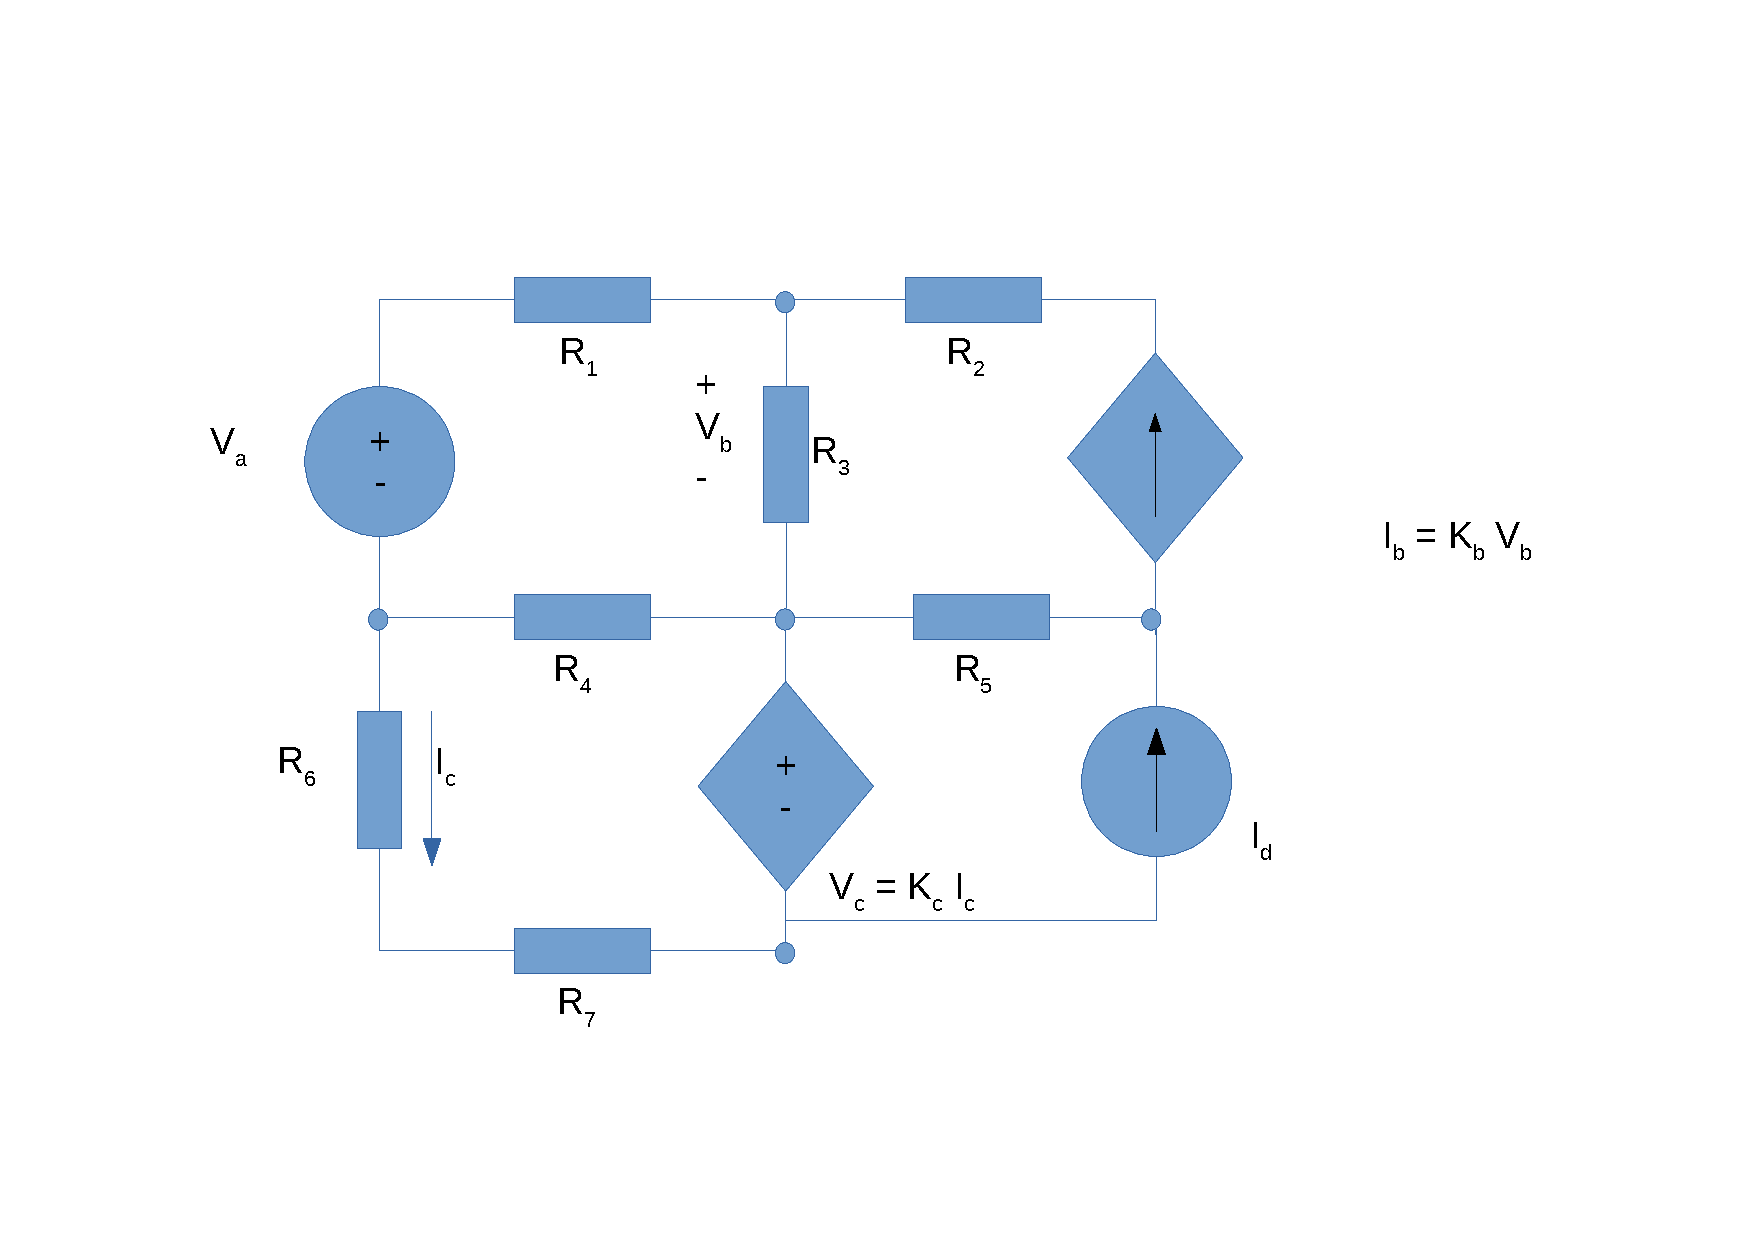
\includegraphics[scale=0.8]{circuito}
\caption{Final circuit}
\label{fig:circuito}
\end{figure}

The individual costs of the components used: \par
- Diodes - cost: 2.3MU; \par
- Capacitor - 5MU; \par
- Resistances - 55MU. \par

The data used was the following:

\begin{center}
  \begin{tabular}{ | c | c | }
    \hline    
    {\bf Name} & {\bf Value [F, V, $\Omega$ or S]} \\ \hline
    $R_1$ & 1.04765357286e3 \\ \hline 
    $R_2$ & 2.06140068334e3 \\ \hline 
    $R_3$ & 3.03459085363e3 \\ \hline 
    $R_4$ & 4.00398818216e3 \\ \hline 
    $R_5$ & 3.11499853456e3 \\ \hline 
    $R_6$ & 2.04588646991e3 \\ \hline 
    $R_7$ & 1.04390152967e3 \\ \hline 
    $V_s$ & 5.02522591213 \\ \hline 
    $C$ & 1.00982536324e-6 \\ \hline
    $K_b$ & 7.28209304852e-3 \\ \hline
    $K_c$ & 8.36641247715e3 \\ 
    \hline
  \end{tabular}
\end{center}





\section{Theoretical Analysis}
\label{sec:analysis}

\subsection{Question 1: Node Analysis}
This preliminary analysis of the circuit is the basis of the rest of the work and to do this we used the nodal method in the same way as used in T1. We have the equations: (the nomenclature for all nodes and branches is present in figure 1).\par
\emph{Node 0 (ground):}
\begin{equation}
    \frac{1}{R_1}(V_2-V_1) + \frac{1}{R_4}(V_5-0)- I_d  = 0
\end{equation}\par

\emph{Node 2:}
\begin{equation}
    \frac{1}{R_1}(V_1-V_2) + \frac{1}{R_2}(V_3-V_2) + \frac{1}{R_3}(V_5-V_2) = 0
\end{equation}\par

\emph{Node 3:}
\begin{equation}
    \frac{1}{R_2}(V_2-V_3) + I_b  = 0
\end{equation}\par

\emph{Node 5:}
\begin{equation}
    \frac{1}{R_3}(V_2-V_5) + \frac{1}{R_5}(V_6-V_5) + \frac{1}{R_4}(0-V_5) - I_d = 0
\end{equation}\par

\emph{Node 6:}
\begin{equation}
    \frac{1}{R_5}(V_5-V_6) - I_b - I_c = 0
\end{equation}\par

\emph{Node 7:}
\begin{equation}
    \frac{1}{R_6}(V_7-0) + I_d  = 0
\end{equation}\par

\emph{Node 8:}
\begin{equation}
    \frac{1}{R_7}(V_7-V_8) - I_d + I_c = 0
\end{equation}\par

\emph{Additional equation:}
\begin{equation}
     V_5 - V_8 - K_dI_d = 0
\end{equation}\par

\emph{Additional equation:}
\begin{equation}
     V_2 - V_5 - \frac{I_b}{K_b} = 0
\end{equation}\par

And the results are shown in the following table:

\begin{center}
  \begin{tabular}{ | c | c | }
    \hline    
    {\bf Name} & {\bf Value [A or V]} \\ \hline
    $V_1$ & 5.025226e+00 \\ \hline 
$V_2$ & 4.724476e+00 \\ \hline 
$V_3$ & 4.104661e+00 \\ \hline 
$V_5$ & 4.765766e+00 \\ \hline 
$V_6$ & 5.702373e+00 \\ \hline 
$V_7$ & -1.847813e+00 \\ \hline 
$V_8$ & -2.790649e+00 \\ \hline 
$I_1$ & -2.870701e-04 \\ \hline 
$I_2$ & -3.006765e-04 \\ \hline 
$I_3$ & 1.360640e-05 \\ \hline 
$I_4$ & 1.190255e-03 \\ \hline 
$I_5$ & 3.006765e-04 \\ \hline 
$I_6$ & 9.031846e-04 \\ \hline 
$I_7$ & 9.031846e-04 \\ \hline 
$I_s$ & -2.870701e-04 \\ \hline 
$I_d$ & 9.031846e-04 \\ \hline 
$I_b$ & -3.006765e-04 \\ \hline 
$I_c$ & -2.168404e-19 \\ 

    \hline
  \end{tabular}
\end{center}
All the variables preceded by I are currents and are expressed in Ampere, the other variables, preceeded by V are voltages and are expressed in Volt.



\subsection{Question 2: Equivalent Resistance ($R_{eq}$)}
The resolution of this question was based on the suggestion presented. Firstly, we set $V_s =0$ and replaced the capacitor by a voltage source $V_x = V_6 - V_8$ and ran the nodal analysis in order to obtain the current $I_x$ witch is the current supplied by $V_x$.\par
Then, with the equation: 
\begin{equation}
     R_{eq} = \frac{V_x}{I_x}
\end{equation}\par
We obtain the Equivalent resistance. \par 
The time constant $\tau$ is calculated by doing $\tau=R_{eq}C$\par
 Since the capacitor was replaced by a Voltage source witch terminals have the same difference of potential as $V_6 - V_8$ in Question 1, this is a known variable that corresponds to $V_x$ ($V_{eq}$). $I_x$ can also be obtainned by running the nodal method with $V_s = 0$. We needed to do this because there is no faster way to calculate the Equivalent Resistance in a circuit where there are resistances in paralell, in series and a capacitor. Basically, the procedure was based on \emph{Thévenin} theorem to obtain $V_{eq}$. By doing this, we have $V_{eq}=R_{eq}I_x$, where $R_{eq}$ is the only unknown variable. \par

The results:

\begin{center}
  \begin{tabular}{ | c | c | }
    \hline    
    {\bf Name} & {\bf Value [A or V]} \\ \hline
    $V_x$ & 8.493021e+00 \\ \hline 
$V_1$ & 0.000000e+00 \\ \hline 
$V_2$ & 0.000000e+00 \\ \hline 
$V_3$ & -0.000000e+00 \\ \hline 
$V_5$ & 0.000000e+00 \\ \hline 
$V_6$ & 8.493021e+00 \\ \hline 
$V_7$ & 0.000000e+00 \\ \hline 
$V_8$ & 0.000000e+00 \\ \hline 
$I_1$ & 0.000000e+00 \\ \hline 
$I_2$ & 0.000000e+00 \\ \hline 
$I_3$ & 0.000000e+00 \\ \hline 
$I_4$ & 0.000000e+00 \\ \hline 
$I_5$ & 2.726493e-03 \\ \hline 
$I_6$ & -0.000000e+00 \\ \hline 
$I_7$ & -0.000000e+00 \\ \hline 
$I_s$ & 0.000000e+00 \\ \hline 
$I_d$ & -0.000000e+00 \\ \hline 
$I_b$ & 0.000000e+00 \\ \hline 
$I_x$ & 2.726493e-03 \\ \hline 
$Req (kOhm)$ & 3.114999e+00 \\ \hline 
$tau (ms)$ & 3.145605e+00 \\ 

    \hline
  \end{tabular}
\end{center}


\subsection{Question 3: Natural solution $v_{6t}(t)$}
The natural solution $v_{6t}(t)$ can be obtained in the interval $[0,20]ms$, by doing: \par
\begin{equation}
     V_6(t) = V_{6n}(t) + V_{6f}(t)
\end{equation}\par
Where:\par
\begin{equation}
     V_{6n}(t) = {A}e^{\frac{-t}{\tau}}
\end{equation}\par
And $v_{6f}(t=0s)$ because $v_s(t=0s)=0$\par
Then:
\begin{equation}
     V_6(0) = V_x(0) + V_8(0)
\end{equation}\par
So ($v_8(t=0s)=0$):
\begin{equation}
     V_6(0) = V_x(0) 
\end{equation}\par
Finally, we get the natural solution:
\begin{equation}
     V_x =  {A}e^{\frac{-t}{\tau}}
\end{equation}\par

By doing this, the plot obtained is the one shown below:

\begin{figure}[H] \centering
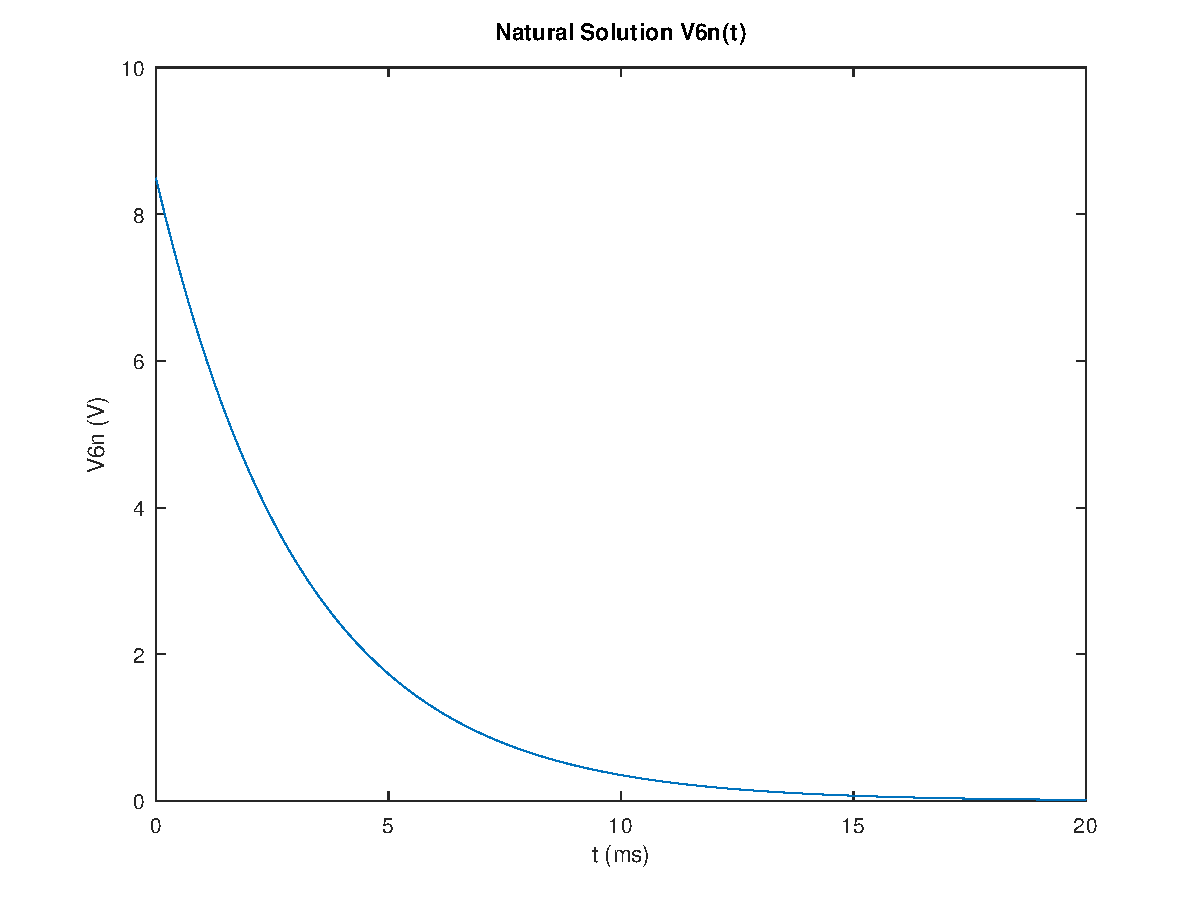
\includegraphics[width=0.7\linewidth]{../mat/alinea3.pdf}
\caption{Natural solution $v_{6t}(t)$}
\label{fig:plot3}
\end{figure}


\subsection{Question 4: Forced solution $v_{6f}(t)$ (f=1Khz)}
In this question, we have used a phasor voltage source $V_s = 1$, since $\phi = 0$, we get:
\begin{equation}
     v_s = sen(2\pi ft) => v_s = -(sen(\phi_s) + icos(\phi_s))
\end{equation}\par
So, $v_s=-i$.
\begin{equation}
     Z_c = \frac{1}{j\omega c}
\end{equation}\par
Where $\omega= 2\pi f$ and $f= 1000Hz$.\par

Then, replacing C with  impedance $Z_c$ and running the nodal analysis to determine the phasor voltages in all nodes we have the following results:\par

\begin{center}
  \begin{tabular}{ | c | c | }
    \hline    
    {\bf Name} & {\bf Value [V]} \\ \hline
    $V_1$ & -0.000000e+00 \\ \hline 
$V_2$ & 3.924207e-19 \\ \hline 
$V_3$ & 6.411465e-19 \\ \hline 
$V_5$ & 3.758515e-19 \\ \hline 
$V_6$ & -8.529278e-02 \\ \hline 
$V_7$ & -9.190910e-20 \\ \hline 
$V_8$ & -0.000000e+00 \\ 

    \hline
  \end{tabular}
\end{center}

We have calculated the module of $V_6$ with "abs" Octave's function. Then, the phase is calculated in the expression:
\begin{equation}
     phase_6 = 0 + arctan({2\pi f}{R_{eq}}{C})
\end{equation}\par

Where $R_{eq}$ and $C$ are the equivalent resistance and the Capacitor's capacitance, respectively.

And, finnaly, the forced solution is given by the expression:
\begin{equation}
     V_{6f}= V_6cos({2\pi f}{t} - phase_6)
\end{equation}\par
and the following plot:\par

\begin{figure}[H] \centering
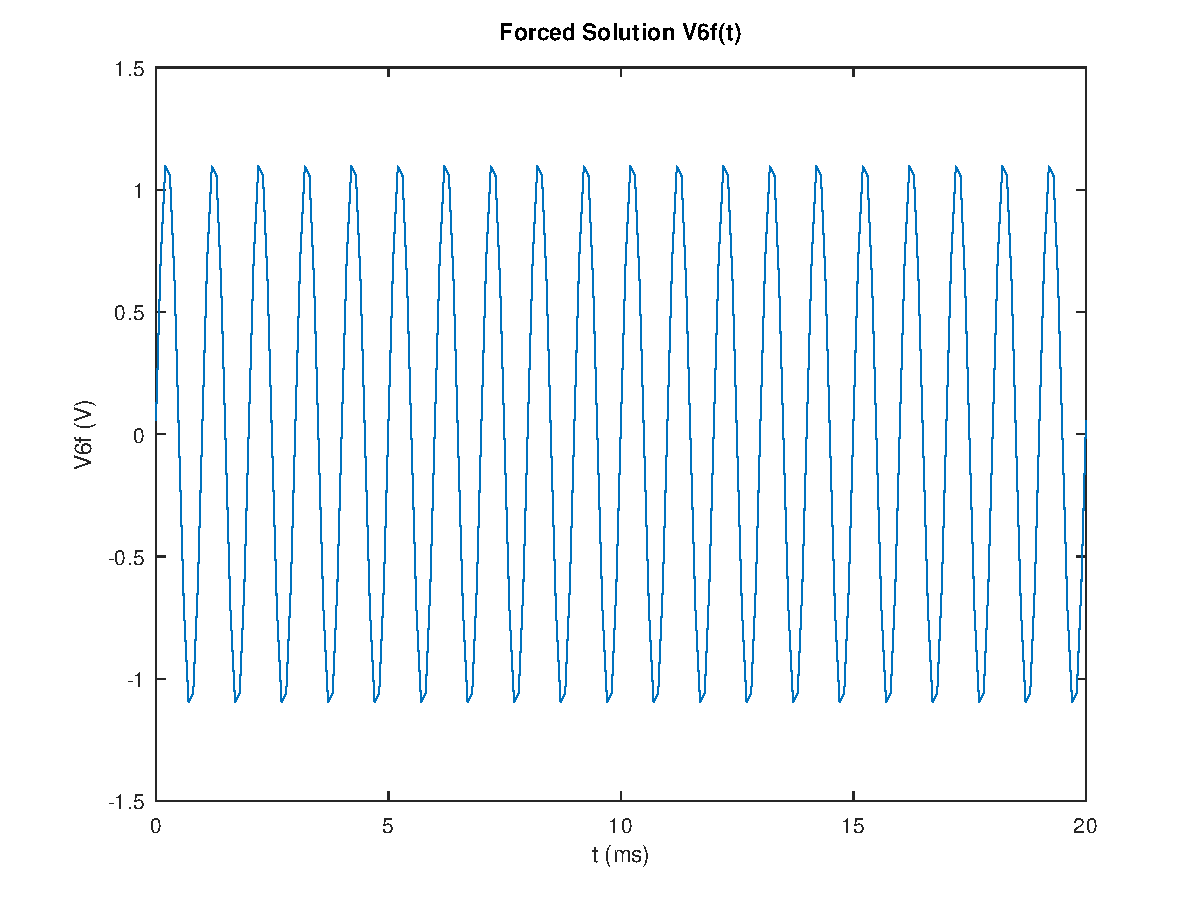
\includegraphics[width=0.7\linewidth]{../mat/alinea4.pdf}
\caption{Forced solution $v_{6t}(t)$}
\label{fig:plot4}
\end{figure}

where $V_6$ is the module value, calculated in the previous expression.



\subsection{Question 5: Final solution $v_{6}(t)$ }
The final total solution is given by:
\begin{equation}
     V_6(t) = V_{6n}(t) + V_{6f}(t)
\end{equation}\par
Considering the time period of $[0 ; 20]ms$: \par $v_s = sin(2\pi ft)$ and $v_6(t)= v_{6n}(t) + v_{6f}(t)$
Considering the time period of $[-5,0]ms$ (In this period of time there is no variation of $v_s$ and so, $v_6$ is also constant, as seen before):\par $v_s = V_s (initial value)$ and $v_6(t) =V_6$.\par
The results ($v_6(t) - blue, v_6 (t) - red$):
\begin{figure}[H] \centering
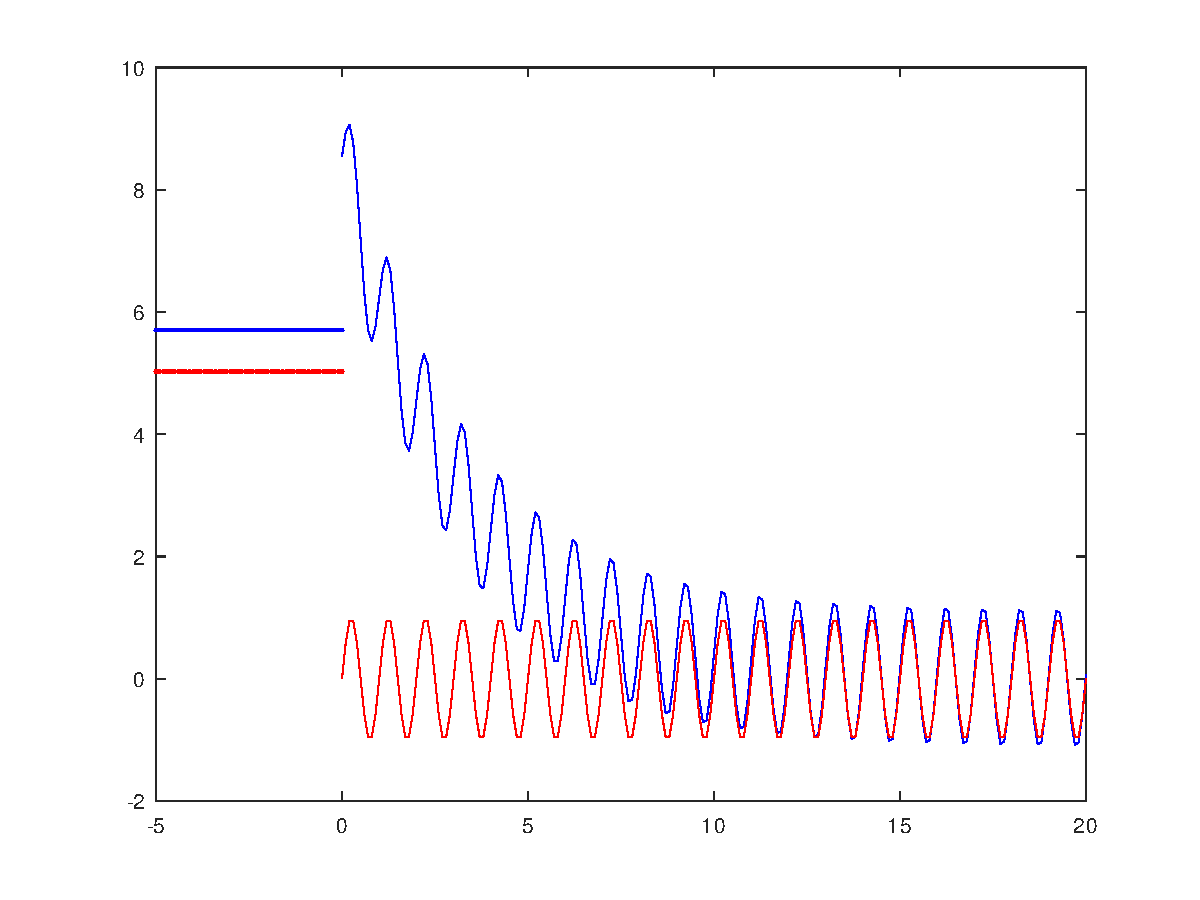
\includegraphics[width=0.7\linewidth]{../mat/alinea5.pdf}
\caption{Final solution $v_{6}(t)$}
\label{fig:plot5}
\end{figure}

\subsection{Question 6: Frequency response}
The main focus of this procedure was to determine the frequency response $v_6(f)$, $v_c(f)$ and $v_s(f)$ for a frequency range of 0.1Hz to 1Mhz (using logarithmic scale for f). \par
As mention before, the impedance expression is:
\begin{equation}
     Z_c = \frac{1}{j\omega c}
\end{equation}\par
Then, we ran the nodal analysis (like in question 4) for each value of frequency determining the phaser voltage in each node, which allowed us to determine the $v_6(f)$, $v_c(f) = v_6(f) - v_8(f)$ and $v_s(f)$ values. As seen before, the phasor voltage $v_s$ value is independet from he frequency and so, it is constant ($v_s = -i$). \par
We have used the magnitude values in dB and phase in degrees, in order to represent the results:\par
\begin{equation}
     magnitude (dB) = 20log_{10}(abs(x))
\end{equation}\par
And,
\begin{equation}
     phase (degrees) = \frac{180}{\pi}angle(x)
\end{equation}\par
where x is the phasor voltage.\par
The $v_s$ is the \textcolor{blue}{blue} line, $v_c$ \textcolor{green}{green} and the $v_6$ the \textcolor{red}{red} one.\par
The results are shown in the following plots:

\begin{figure}[H] \centering
\includegraphics[width=0.7\linewidth]{../mat/alinea61.pdf}
\caption{Magnitude of phasor voltages ($dB$)}
\label{fig:plot6}
\end{figure}

\begin{figure}[H] \centering
\includegraphics[width=0.7\linewidth]{../mat/alinea62.pdf}
\caption{Phase of phasor voltages (degrees)}
\label{fig:plot7}
\end{figure}







\section{Simulation Analysis}
\label{sec:simulation}

\subsection{Operating Point Analysis}

Table~\ref{tab:op} shows the simulated operating point results for the circuit
under analysis. Compared to the theoretical analysis results, one notices the
following differences: describe and explain the differences.

\begin{table}[h]
  \centering
  \begin{tabular}{|l|r|}
    \hline    
    {\bf Name} & {\bf Value [A or V]} \\ \hline
    @g0[i] & -2.62010e-04\\ \hline
@id[current] & 1.039703e-03\\ \hline
@r1[i] & 2.500671e-04\\ \hline
@r2[i] & -2.62010e-04\\ \hline
@r3[i] & -1.19432e-05\\ \hline
@r4[i] & 1.159730e-03\\ \hline
@r5[i] & -1.30171e-03\\ \hline
@r6[i] & 9.096634e-04\\ \hline
@r7[i] & 9.096634e-04\\ \hline
n1 & 5.046111e+00\\ \hline
n2 & 4.787759e+00\\ \hline
n3 & 4.248290e+00\\ \hline
n4 & -1.88445e+00\\ \hline
n5 & 4.824275e+00\\ \hline
n6 & 8.832281e+00\\ \hline
n8 & -2.81232e+00\\ \hline
n9 & -1.88445e+00\\ \hline

  \end{tabular}
  \caption{Operating point. A variable preceded by @ is of type {\em current}
    and expressed in Ampere; other variables are of type {\it voltage} and expressed in
    Volt.}
  \label{tab:op}
\end{table}

\lipsum[1-1]


\subsection{Transient Analysis}

Figure~\ref{fig:trans} shows the simulated transient analysis results for the
circuit under analysis. Compared to the theoretical analysis results, one
notices the following differences: describe and explain the differences.

\lipsum[1-1]



\subsection{Frequency Analysis}

\subsubsection{Magnitude Response}

Figure~\ref{fig:acm} shows the magnitude of the frequency response for the
circuit under analysis. Compared to the theoretical analysis results, one
notices the following differences: describe and explain the differences.

\lipsum[1-1]

\subsubsection{Phase Response}

Figure~\ref{fig:acp} shows the magnitude of the frequency response for the
circuit under analysis. Compared to the theoretical analysis results, one
notices the following differences: describe and explain the differences.


\lipsum[1-1]

\subsubsection{Input Impedance}

Figure~\ref{fig:zim} shows the magnitude of the frequency response for the
circuit under analysis. Compared to the theoretical analysis results, one
notices the following differences: describe and explain the differences.


\lipsum[1-1]





\section{Conclusion}
\label{sec:conclusion}

Summing up, in this laboratory assignment (T2) we have made both theoretical analysis as well as simulations of several different but similar and correlated circuits. \par
The results obtained in both analysis were either put in a table or plotted in order to make comparations between the theoretical and simulation analysis.
The reasoning behind these results is that we studied a very simple circuit containing only linear components. If the components used were more complex, the case would not be the same and we could detect real differences between the values calculated and simulated. \par
That being said we would like to end this report by presenting both the theoretical and simulation results side by side in order to easily compare the results.


\begin{figure}[H]
    \minipage{0.50\textwidth}
      \centering
      \begin{tabular}{ | c | c | }
      \hline    
      {\bf Name} & {\bf Value [A or V]} \\ \hline
      $V_1$ & 5.025226e+00 \\ \hline 
$V_2$ & 4.724476e+00 \\ \hline 
$V_3$ & 4.104661e+00 \\ \hline 
$V_5$ & 4.765766e+00 \\ \hline 
$V_6$ & 5.702373e+00 \\ \hline 
$V_7$ & -1.847813e+00 \\ \hline 
$V_8$ & -2.790649e+00 \\ \hline 
$I_1$ & -2.870701e-04 \\ \hline 
$I_2$ & -3.006765e-04 \\ \hline 
$I_3$ & 1.360640e-05 \\ \hline 
$I_4$ & 1.190255e-03 \\ \hline 
$I_5$ & 3.006765e-04 \\ \hline 
$I_6$ & 9.031846e-04 \\ \hline 
$I_7$ & 9.031846e-04 \\ \hline 
$I_s$ & -2.870701e-04 \\ \hline 
$I_d$ & 9.031846e-04 \\ \hline 
$I_b$ & -3.006765e-04 \\ \hline 
$I_c$ & -2.168404e-19 \\ 

      \hline
      \end{tabular}
      \caption{Theoretical Question 1}
    \endminipage\hfill
    \minipage{0.50\textwidth}
      \centering
      \begin{tabular}{ | c | c | }
      \hline    
      {\bf Name} & {\bf Value [A or V]} \\ \hline
      @c0[i] & 0.000000e+00\\ \hline
@g0[i] & -3.00677e-04\\ \hline
@r1[i] & 2.870701e-04\\ \hline
@r2[i] & -3.00677e-04\\ \hline
@r3[i] & -1.36064e-05\\ \hline
@r4[i] & 1.190255e-03\\ \hline
@r5[i] & -3.00677e-04\\ \hline
@r6[i] & 9.031846e-04\\ \hline
@r7[i] & 9.031846e-04\\ \hline
n1 & 5.025226e+00\\ \hline
n2 & 4.724476e+00\\ \hline
n3 & 4.104661e+00\\ \hline
n5 & 4.765766e+00\\ \hline
n6 & 5.702373e+00\\ \hline
n7 & -1.84781e+00\\ \hline
n8 & -2.79065e+00\\ \hline
n9 & -2.79065e+00\\ \hline

      \end{tabular}
      \caption{Simulation Question 1}
    \endminipage\hfill
\end{figure}

\begin{figure}[H]
    \minipage{0.50\textwidth}
      \centering
      \begin{tabular}{ | c | c | }
      \hline    
      {\bf Name} & {\bf Value [A or V]} \\ \hline
      $V_x$ & 8.493021e+00 \\ \hline 
$V_1$ & 0.000000e+00 \\ \hline 
$V_2$ & 0.000000e+00 \\ \hline 
$V_3$ & -0.000000e+00 \\ \hline 
$V_5$ & 0.000000e+00 \\ \hline 
$V_6$ & 8.493021e+00 \\ \hline 
$V_7$ & 0.000000e+00 \\ \hline 
$V_8$ & 0.000000e+00 \\ \hline 
$I_1$ & 0.000000e+00 \\ \hline 
$I_2$ & 0.000000e+00 \\ \hline 
$I_3$ & 0.000000e+00 \\ \hline 
$I_4$ & 0.000000e+00 \\ \hline 
$I_5$ & 2.726493e-03 \\ \hline 
$I_6$ & -0.000000e+00 \\ \hline 
$I_7$ & -0.000000e+00 \\ \hline 
$I_s$ & 0.000000e+00 \\ \hline 
$I_d$ & -0.000000e+00 \\ \hline 
$I_b$ & 0.000000e+00 \\ \hline 
$I_x$ & 2.726493e-03 \\ \hline 
$Req (kOhm)$ & 3.114999e+00 \\ \hline 
$tau (ms)$ & 3.145605e+00 \\ 

      \hline
      \end{tabular}
      \caption{Theoretical Question 2}
    \endminipage\hfill
    \minipage{0.50\textwidth}
      \centering
      \begin{tabular}{ | c | c | }
      \hline    
      {\bf Name} & {\bf Value [A or V]} \\ \hline
      @g0[i] & 0.000000e+00\\ \hline
@r1[i] & 0.000000e+00\\ \hline
@r2[i] & 0.000000e+00\\ \hline
@r3[i] & 0.000000e+00\\ \hline
@r4[i] & 0.000000e+00\\ \hline
@r5[i] & 2.726492e-03\\ \hline
@r6[i] & 0.000000e+00\\ \hline
@r7[i] & 0.000000e+00\\ \hline
n1 & 0.000000e+00\\ \hline
n2 & 0.000000e+00\\ \hline
n3 & 0.000000e+00\\ \hline
n5 & 0.000000e+00\\ \hline
n6 & -8.49302e+00\\ \hline
n7 & 0.000000e+00\\ \hline
n8 & 0.000000e+00\\ \hline
n9 & 0.000000e+00\\ \hline

      \end{tabular}
      \caption{Simulation Question 2}
    \endminipage\hfill
\end{figure}

\begin{figure}[H]
    \minipage{0.45\textwidth}
      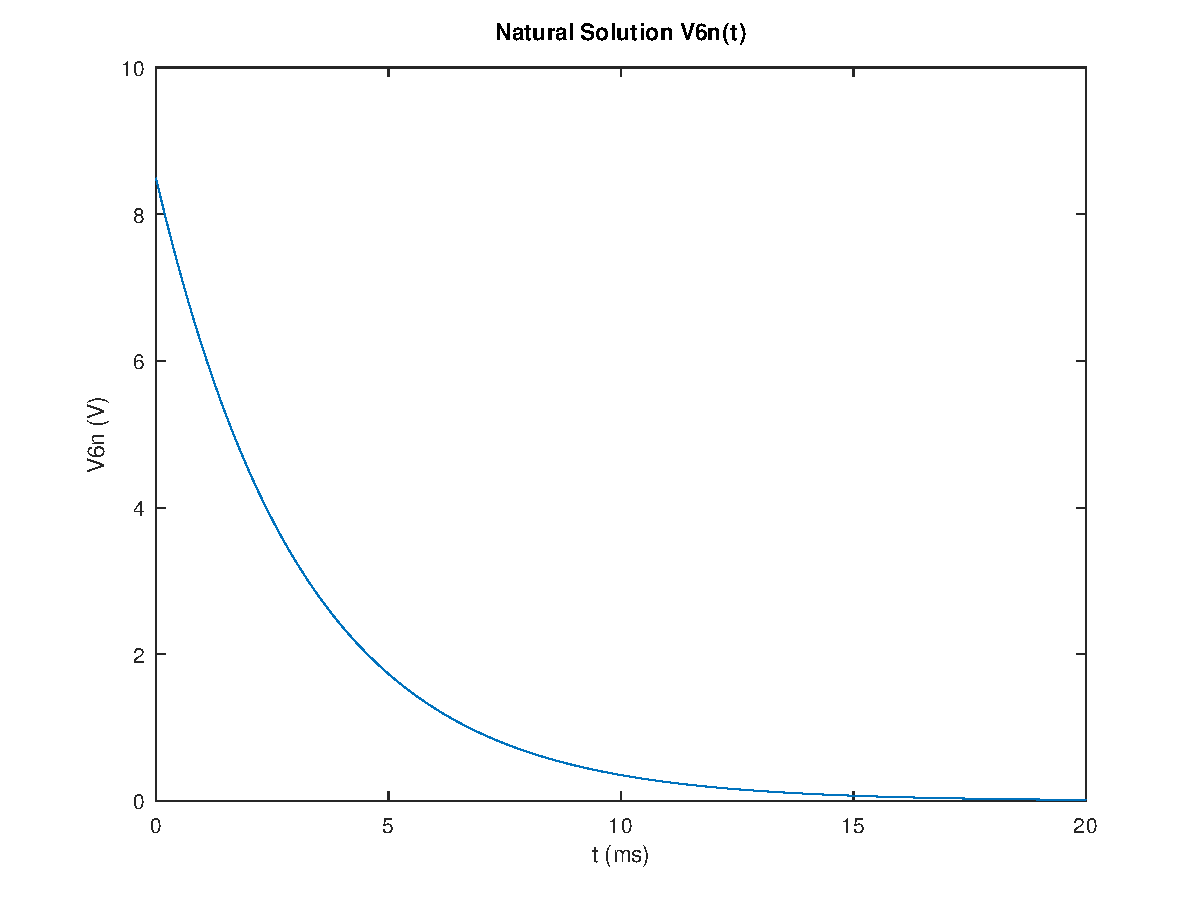
\includegraphics[width=\linewidth]{../mat/alinea3.pdf}
      \caption{Theoretical Question 3}
    \endminipage\hfill
    \minipage{0.45\textwidth}
      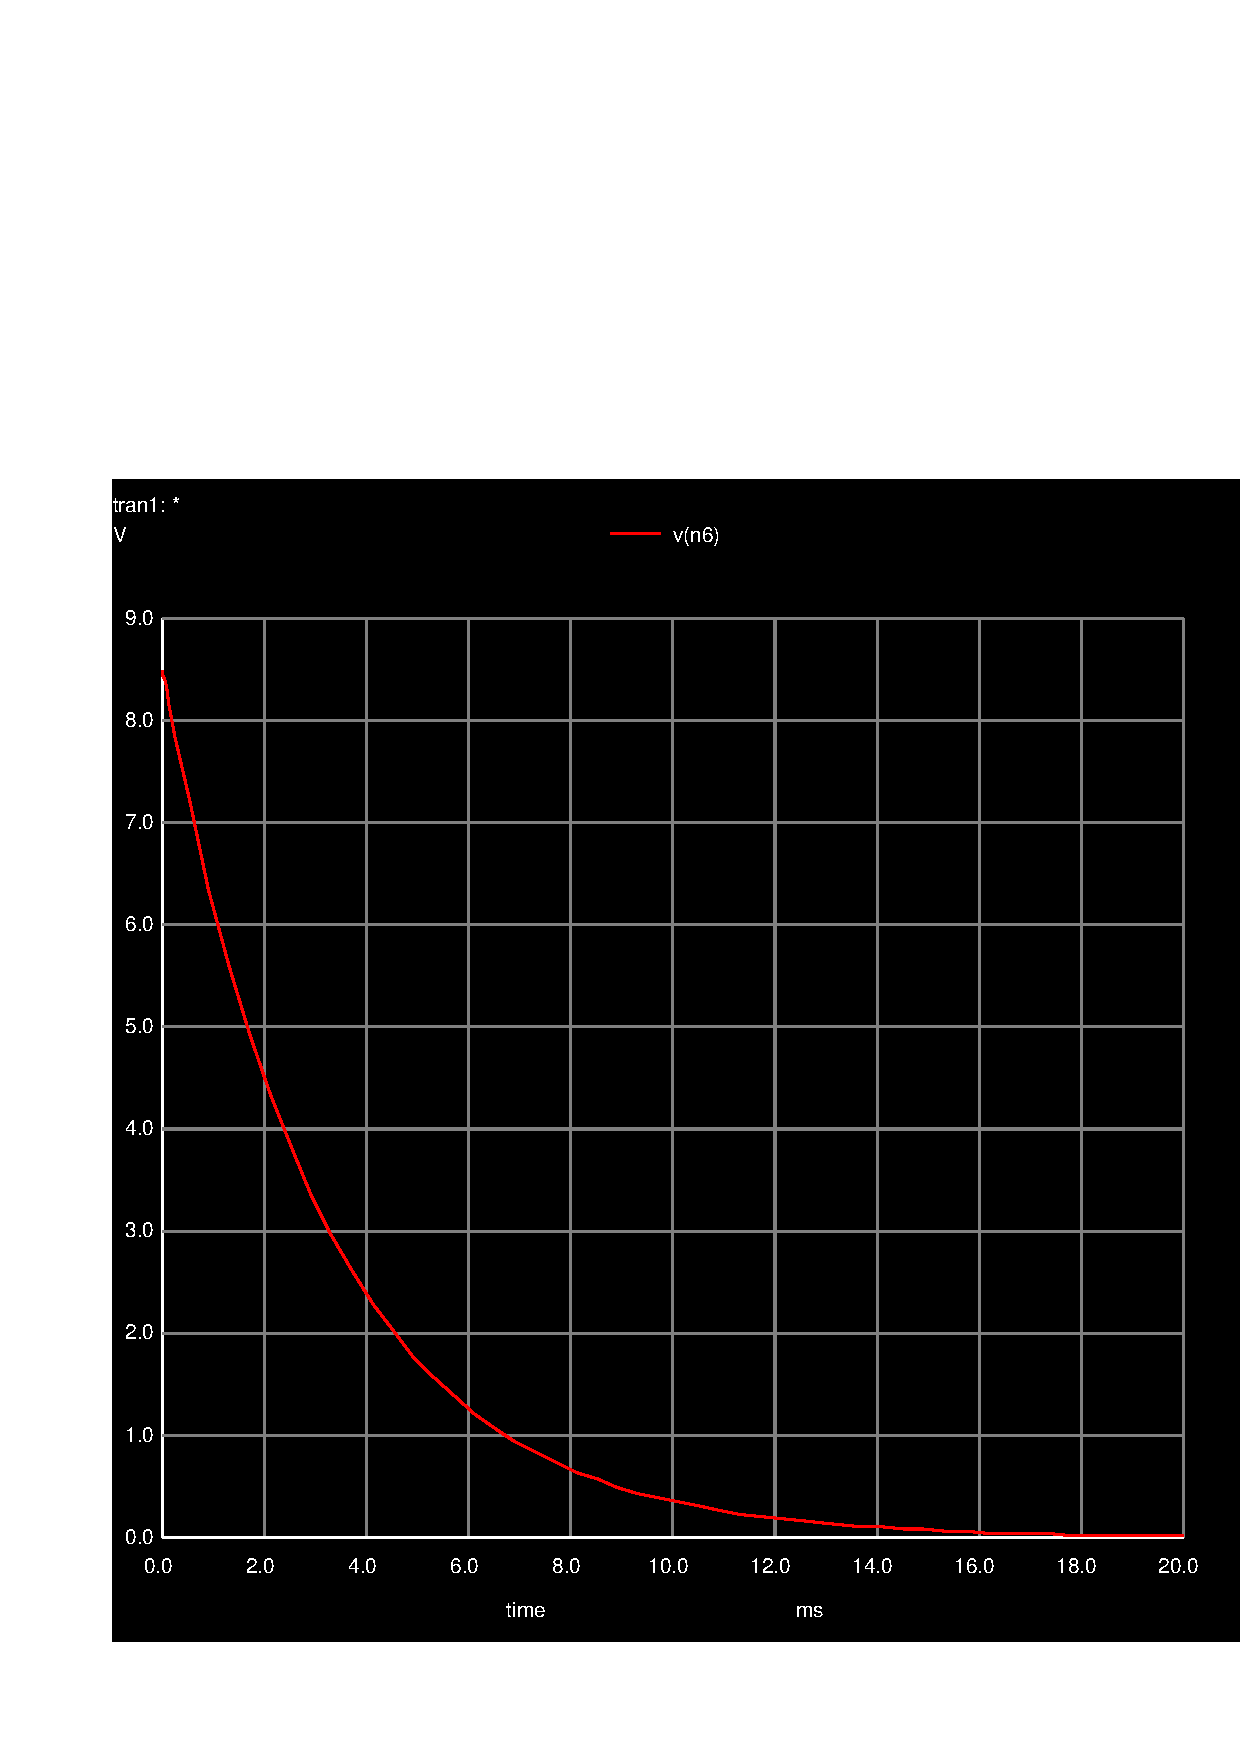
\includegraphics[width=\linewidth]{../sim/transient3.pdf}
      \caption{Simulation Question 3}
    \endminipage\hfill
\end{figure}

\begin{figure}[H]
    \minipage{0.45\textwidth}
      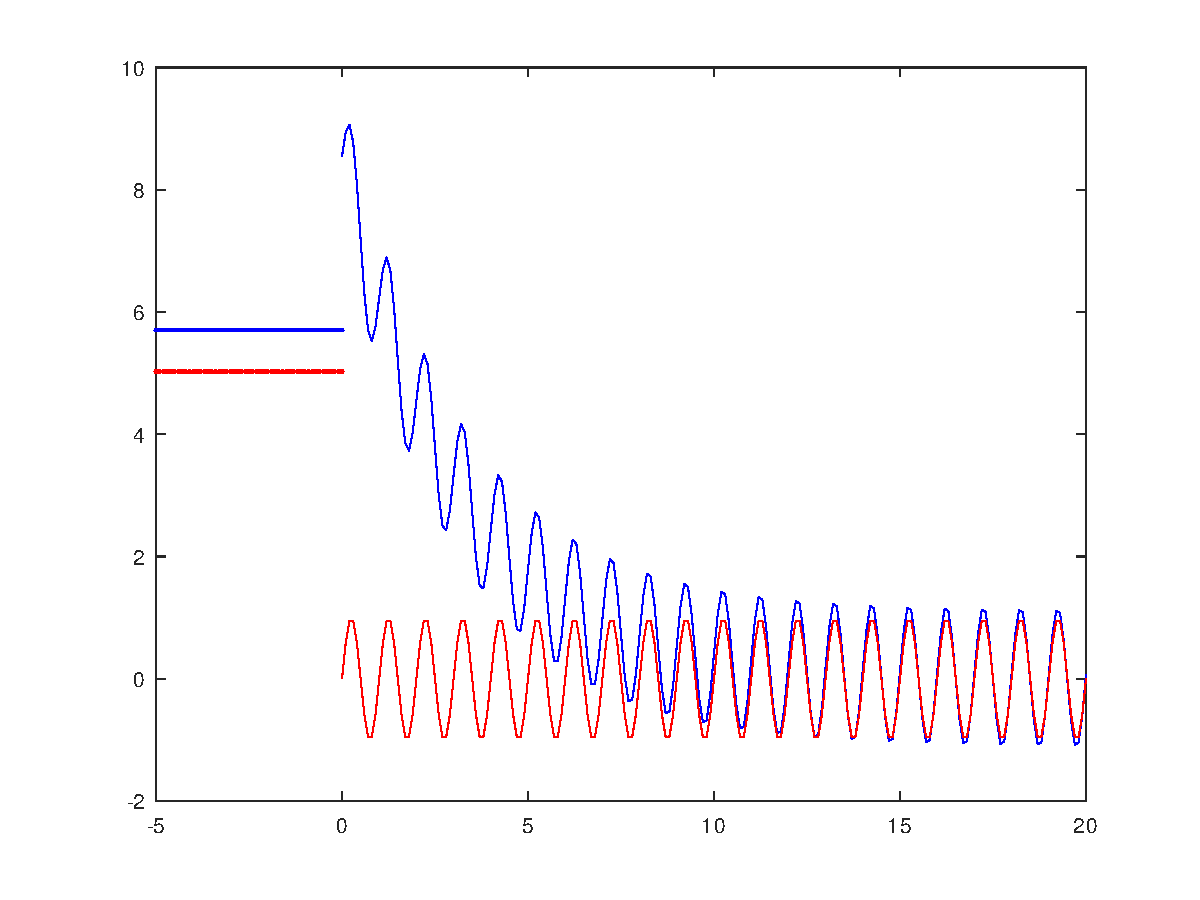
\includegraphics[width=\linewidth]{../mat/alinea5.pdf}
      \caption{Theoretical Question 5}
    \endminipage\hfill
    \minipage{0.45\textwidth}
      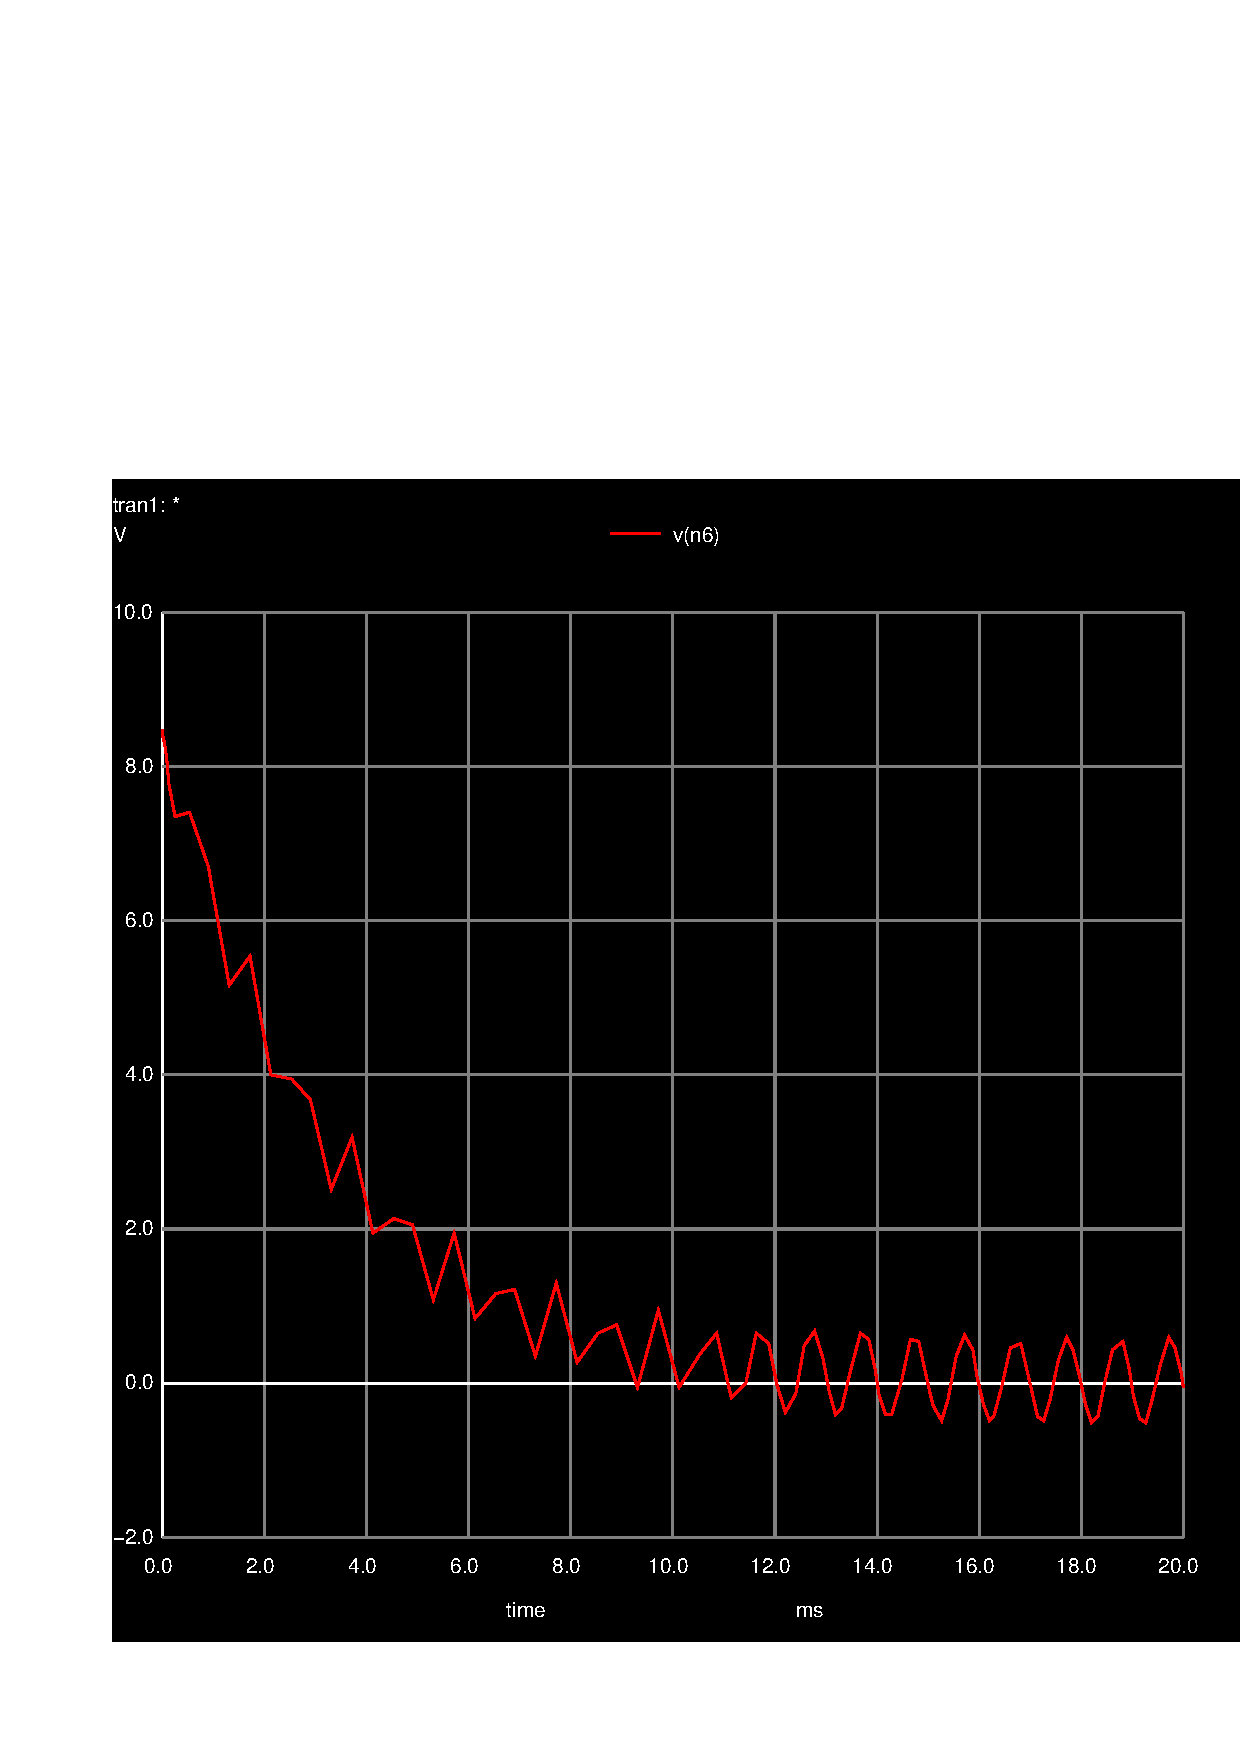
\includegraphics[width=\linewidth]{../sim/transient4r.pdf}
      \caption{Simulation Question 4}
    \endminipage\hfill
\end{figure}

\begin{figure}[H]
    \minipage{0.45\textwidth}
      \includegraphics[width=\linewidth]{../mat/alinea61.pdf}
      \caption{Theoretical Question 6 - Frequency Response}
    \endminipage\hfill
    \minipage{0.45\textwidth}
      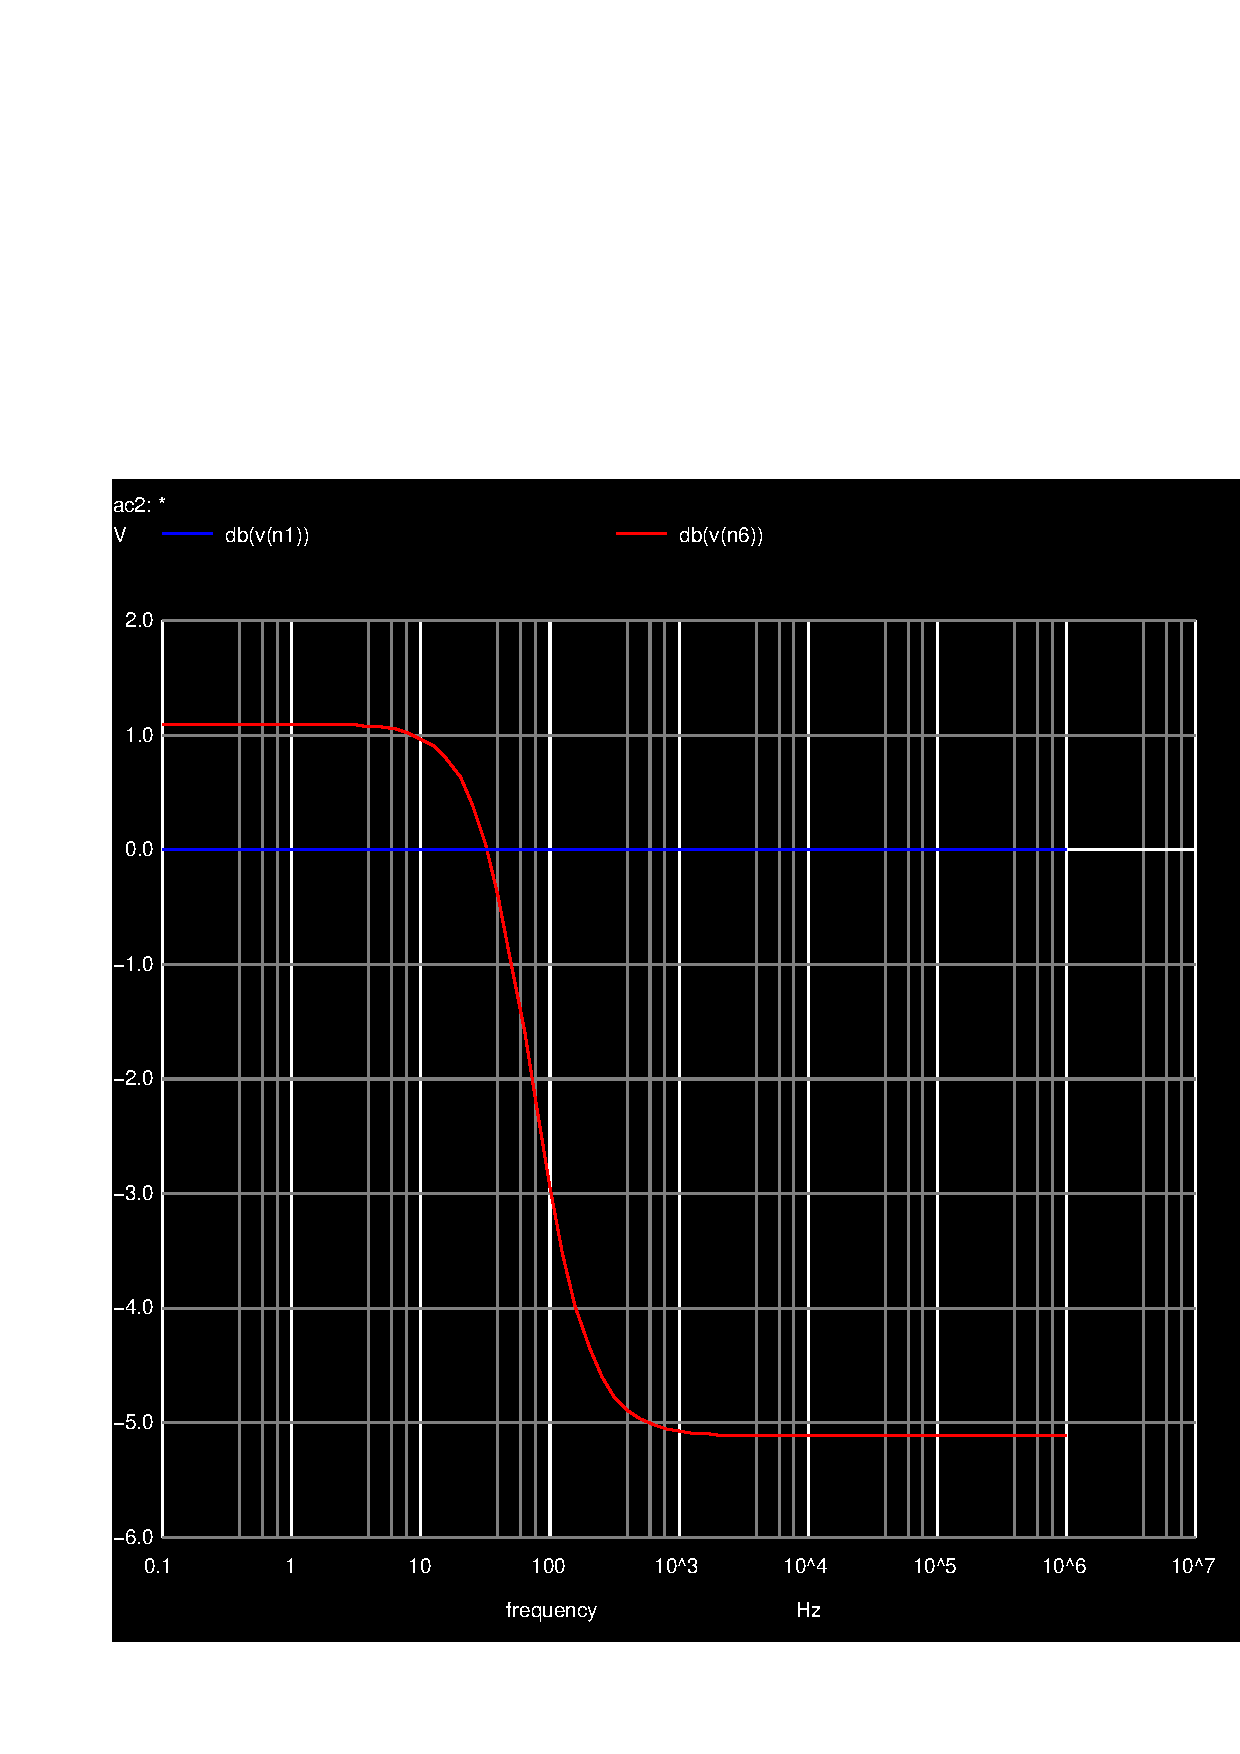
\includegraphics[width=\linewidth]{../sim/fresponse.pdf}
      \caption{Simulation Question 5 - Frequency Response}
    \endminipage\hfill
\end{figure}

%\cleardoublepage

% ----------------------------------------------------------------------
%  Bibliography
% ----------------------------------------------------------------------
%\addcontentsline{toc}{section}{\bibname}
%\bibliographystyle{abbrvunsrtnat} % <<<<< SELECT IF USING REFERENCES BY NUMBER (CITATION ORDER)
%\bibliography{../../../BIBfile.bib}

% ----------------------------------------------------------------------
\end{document}
% ----------------------------------------------------------------------

